\newfloat{algo}{h}{alg}

\graphicspath{{chapt_dutch/}{intro/}{chapt2/}{chapt3/}{chapt4/}{chapt5/}{chapt6/}{chapt7/}}

% Header
\renewcommand\evenpagerightmark{{\scshape\small Appendix B}}
\renewcommand\oddpageleftmark{{\scshape\small Details on the online analysis package}}

\renewcommand{\bibname}{References}

\hyphenation{}

\chapter[Details on the offline analysis package]%
{Details on the offline analysis package}
\label{app2}

The data collected in GIF++ thanks to the DAQ described in Appendix~\ref{app1} is difficult to interpret by a human user that doesn't have a clear idea of the raw data architecture of the ROOT data files. In order to render the data human readable, a C++ offline analysis tool was designed to provide users with detector by detector histograms that give a clear overview of the parameters monitored during the data acquisition~\cite{GIFOffline}. In this appendix, details about this software in the context of GIF++, as of how the software was written and how it functions will be given.

\section{GIF++ Offline Analysis file tree}
\label{app2:sec:code}

	GIF++ Offline Analysis source code is fully available on github at \url{https://github.com/afagot/GIF_OfflineAnalysis}. The software requires \href{https://root.cern.ch/downloading-root}{ROOT} as non-optionnal dependency as it takes ROOT files in input and write an output ROOT file containing histograms. To compile the GIF++ Offline Analysis project is compiled with cmake. To compile, first a \textinline{build/} directory must be created to compile from there:\\

	\begin{bashcode}
 mkdir build
 cd build
 cmake ..
 make
 make install
	\end{bashcode}
\vspace{5mm}
	To clean the directory and create a new build directory, the bash script \textinline{cleandir.sh} can be used:\\
	
	\begin{bashcode}
 ./cleandir.sh
	\end{bashcode}
\vspace{5mm}
	The source code tree is provided below along with comments to give an overview of the files' content. The different objects created for this project (\cppinline{Infrastructure}, \cppinline{Trolley}, \cppinline{RPC}, \cppinline{Mapping}, \cppinline{RPCHit}, \cppinline{RPCCluster} and \cppinline{Inifile}) will be described in details in the following sections.\\

	\dirtree{%
	 .1 GIF\_OfflineAnalysis.
	 .2 bin.
	 .3 offlineanalysis\DTcomment{executable}.
	 .2 build\DTcomment{cmake compilation directory}.
	 .3 ....
	 .2 include\DTcomment{list of C++ header files}.
	 .3 Cluster.h\DTcomment{declaration of object RPCCluster}.
	 .3 Current.h\DTcomment{declaration of GetCurrent analysis macro}.
	 .3 GIFTrolley.h\DTcomment{declaration of object Trolley}.
	 .3 Infrastructure.h\DTcomment{declaration of object Infrastructure}.
	 .3 IniFile.h\DTcomment{declaration of object IniFile for ini parser}.
	 .3 Mapping.h\DTcomment{declaration of object Mapping}.
	 .3 MsgSvc.h\DTcomment{declaration of offline log messages}.
	 .3 OfflineAnalysis.h\DTcomment{declaration of data analysis macro}.
	 .3 RPCDetector.h\DTcomment{declaration of object RPC}.
	 .3 RPCHit.h\DTcomment{declararion of object RPCHit}.
	 .3 types.h\DTcomment{definition of useful variable types}.
	 .3 utils.h\DTcomment{declaration of useful functions}.
	 .2 obj\DTcomment{binary files created by compiler}.
	 .3 ....
	 .2 src\DTcomment{list of C++ source files}.
	 .3 Cluster.cc\DTcomment{definition of object RPCCluster}.
	 .3 Current.cc\DTcomment{definition of GetCurrent analysis macro}.
	 .3 GIFTrolley.cc\DTcomment{definition of object Trolley}.
	 .3 Infrastructure.cc\DTcomment{definition of object Infrastructure}.
	 .3 IniFile.cc\DTcomment{definition of object IniFile for ini parser}.
	 .3 main.cc\DTcomment{main file}.
	 .3 Mapping.cc\DTcomment{definition of object Mapping}.
	 .3 MsgSvc.cc\DTcomment{definition of offline log messages}.
	 .3 OfflineAnalysis.cc\DTcomment{definition of data analysis macro}.
	 .3 RPCDetector.cc\DTcomment{definition of object RPC}.
	 .3 RPCHit.cc\DTcomment{definition of object RPCHit}.
	 .3 utils.cc\DTcomment{definition of useful functions}.
	 .2 cleandir.sh\DTcomment{bash script to clean build directory}.
	 .2 CMakeLists.txt\DTcomment{set of instructions for cmake}.
	 .2 config.h.in\DTcomment{definition of version number}.
	 .2 README.md\DTcomment{REAMDE file for github}.
	}
	
\section{Usage of the Offline Analysis}
\label{app2:sec:usage}

	In order to use the Offline Analysis tool, it is necessary to know the Scan number and the HV Step of the run that needs to be analysed. This information needs to be written in the following format:\\
	
	\begin{bashcode}
 Scan00XXXX_HVY
	\end{bashcode}
\vspace{5mm}
	where \textinline{XXXX} is the scan ID and \textinline{Y} is the high voltage step (in case of a high voltage scan, data will be taken for several HV steps). This format corresponds to the base name of data files in the database of the GIF++ webDCS. Usually, the offline analysis tool is automatically called by the webDCS at the end of data taking or by a user from the webDCS panel if an update of the tool was brought. Nontheless, an expert can locally launch the analysis for tests on the GIF++ computer, or a user can get the code on is local machine from github and download data from the webDCS for is own analysis. To launch the code, the following command can be used from the \textinline{GIF_OfflineAnalysis} folder:\\
	
	\begin{bashcode}
 bin/offlineanalysis /path/to/Scan00XXXX_HVY
	\end{bashcode}
\vspace{5mm}
	where, \textinline{/path/to/Scan00XXXX_HVY} refers to the local data files. Then, the offline tool will by itself take care of finding all available ROOT data files present in the folder, as listed bellow:

	\begin{itemize}
		\item[•] \textinline{Scan00XXXX_HVY_DAQ.root} containing the TDC data as described in Appendix~\ref{app1:sec:DataReader} (events, hit and timestamp lists), and
		\item[•] \textinline{Scan00XXXX_HVY_CAEN.root} containing the CAEN mainframe data recorded by the monitoring tool webDCS during data taking (HVs and currents of every HV channels). This file is created independently of the DAQ.
	\end{itemize}
	
	\subsection{Output of the offline tool}
	\label{app2:ssec:output}
	
		\subsubsection{ROOT file}
		\label{app2:sssec:ROOT}
	
	The analysis gives in output ROOT datafiles that are saved into the data folder and called using the naming convention \textinline{Scan00XXXX_HVY_Offline.root}. Inside those, a list of \cppinline{TH1} histograms can be found. Its size will vary as a function of the number of detectors in the setup as each set of histograms is produced detector by detector. For each partition of each chamber, can be found:

	\begin{itemize}
		\item[•] \textinline{Time_Profile_Tt_Sc_p} shows the time profile of all recorded events (number of events per time bin),
		\item[•] \textinline{Hit_Profile_Tt_Sc_p} shows the hit profile of all recorded events (number of events per channel),
		\item[•] \textinline{Hit_Multiplicity_Tt_Sc_p} shows the hit multiplicity (number of hits per event) of all recorded events (number of occurences per multiplicity bin),
		\item[•] \textinline{Strip_Mean_Noise_Tt_Sc_p} shows noise/gamma rate per unit area for each strip in a selected time range. After filters are applied on \textinline{Time_Profile_Tt_Sc_p}, the filtered version of \textinline{Hit_Profile_Tt_Sc_p} is normalised to the total integrated time and active detection area of a single channel,
		\item[•] \textinline{Strip_Activity_Tt_Sc_p} shows noise/gamma activity for each strip (normalised version of previous histogram - strip activity = strip rate / average partition rate),
		\item[•] \textinline{Strip_Homogeneity_Tt_Sc_p} shows the \textit{homogeneity} of a given partition (homogeneity = exp(-strip rates standard deviation(strip rates in partition/average partition rate)) ),
		\item[•] \textinline{mask_Strip_Mean_Noise_Tt_Sc_p} shows noise/gamma rate per unit area for each masked strip in a selected time range. Offline, the user can control the noise/gamma rate and decide to mask the strips that are judged to be noisy or dead. This is done via the \textit{Masking Tool} provided by the webDCS,
		\item[•] \textinline{mask_Strip_Activity_Tt_Sc_p} shows noise/gamma activity per unit area for each masked strip with repect to the average rate of active strips,
		\item[•] \textinline{NoiseCSize_H_Tt_Sc_p} shows noise/gamma cluster size, a cluster being constructed out of adjacent strips giving a signal at the \textit{same time} (hits within a time window of \SI{25}{ns}),
		\item[•] \textinline{NoiseCMult_H_Tt_Sc_p} shows noise/gamma cluster multiplicity (number of reconstructed clusters per event),
		\item[•] \textinline{Chip_Mean_Noise_Tt_Sc_p} shows the same information than \textinline{Strip_Mean_Noise_Tt_Scp} using a different binning (1 chip corresponds to 8 strips),
		\item[•] \textinline{Chip_Activity_Tt_Sc_p} shows the same information than \textinline{Strip_Activity_Tt_Scp} using chip binning,
		\item[•] \textinline{Chip_Homogeneity_Tt_Sc_p} shows the homogeneity of a given partition using chip binning,
		\item[•] \textinline{Beam_Profile_Tt_Sc_p} shows the estimated beam profile when taking efficiency scan. This is obtained by filtering \textinline{Time_Profile_Tt_Sc_p} to only consider the muon peak where the noise/gamma background has been subtracted. The resulting hit profile corresponds to the beam profile on the detector channels,
		\item[•] \textinline{L0_Efficiency_Tt_Sc_p} shows the level 0 efficiency that was estimated \textbf{without} muon tracking,
		\item[•] \textinline{MuonCSize_H_Tt_Sc_p} shows the level 0 muon cluster size that was estimated \textbf{without} muon tracking, and
		\item[•] \textinline{MuonCMult_H_Tt_Sc_p} shows the level 0 muon cluster multiplicity that was estimated \textbf{without} muon tracking.
	\end{itemize}

	In the histogram labels, \textinline{t} stands for the trolley number (1 or 3), \textinline{c} for the chamber slot label in trolley  \textinline{t} and \textinline{p} for the partition label (A, B, C or D depending on the chamber layout) as explained in Chapter~\ref{chapt5:sec:GIFpptests}.\\
	
	In the context of GIF++, an extra script called by the webDCS is called to extract the histograms from the ROOT files. The histograms are then stored in PNG and PDF formats into the corresponding folder (a single folder per HV step, so per ROOT file). the goal is to then display the histograms on the \acf{DQM} page of the webDCS in order for the users to control the quality of the data taking at the end of data taking. An example of histogram organisation is given bellow:\\
	
	\newpage
	
	\dirtree{%
	 .1 Scan001000.
	 .2 Scan001000\_HV1\_DAQ.root.
	 .2 Scan001000\_HV1\_CAEN.root.
	 .2 Scan001000\_HV1\_Offline.root.
	 .2 HV1.
	 .3 DAQ.
	 .4 Beam\_Profile\_T1\_S1\_A.png.
	 .4 Beam\_Profile\_T1\_S1\_A.pdf.
	 .4 Beam\_Profile\_T1\_S1\_B.png.
	 .4 Beam\_Profile\_T1\_S1\_B.pdf.
	 .4 ....
	 .3 CAEN.
	 .4 HVapp\_Example\_RPC1.pdf.
	 .4 HVapp\_Example\_RPC1.png.
	 .4 HVapp\_Example\_RPC1.pdf.
	 .4 HVapp\_Example\_RPC1.png.
	 .4 ....
	 .2 Scan001000\_HV2\_DAQ.root.
	 .2 Scan001000\_HV2\_CAEN.root.
	 .2 Scan001000\_HV2\_Offline.root.
	 .2 HV2.
	 .3 DAQ.
	 .4 ....
	 .3 CAEN.
	 .4 ....
	 .2 Scan001000\_HV3\_DAQ.root.
	 .2 Scan001000\_HV3\_CAEN.root.
	 .2 Scan001000\_HV3\_Offline.root.
	 .2 HV3.
	 .3 ....
	 .2 ....
	}
	\vspace{5mm}
	\textbf{\textit{Here can put some screens from the webDCS to show the DQM and the plots available to users.\\}}
	
		\subsubsection{CSV files}
		\label{app2:sssec:CSV}

	Moreover, up to 3 CSV files can be created depending on which ones of the 3 input files were in the data folder:

	\begin{itemize}
		\item[•] \textinline{Offline-Corrupted.csv} , is used to keep track of the amount of data that was corrupted and removed from old data format files that don't contain any data quality flag.
		\item[•] \textinline{Offline-Current.csv} , contains the summary of the currents and voltages applied on each RPC HV channel.
		\item[•] \textinline{Offline-L0-EffCl.csv} , is used to write the efficiencies, cluster size and cluster multiplicity of efficiency runs. Note that \textinline{L0} refers here to \textit{Level 0} and means that the results of effiency and clusterization are a first approximation calculated without performing any muon tracking in between the different detectors. This offline tool provides the user with a preliminar calculation of the efficiency and of the muon event parameters. Another analysis software especially dedicated to muon tracking is called on selected data to retrieve the results of efficiency and muon clusterization using a tracking algorithm to discriminate noise or gamma from muons as muons are the only particles that pass through the full setup, leaving hits than can be used to reconstruct their tracks.
		\item[•] \textinline{Offline-Rate.csv} , is used to write the noise or gamma rates measured in the detector readout partitions.
	\end{itemize}
	
	Note that these 4 CSV files are created along with their \textit{headers} (\textinline{Offline-[...]-Header.csv} containing the names of each data columns) and are automatically merged together when the offline analysis tool is called from the webDCS, contrary to the case where the tool is runned locally from the terminal as the merging bash script is then not called. Thus, the resulting files, used to make official plots, are:

	\begin{itemize}
		\item[•] \textinline{Corrupted.csv} ,
		\item[•] \textinline{Current.csv} ,
		\item[•] \textinline{L0-EffCl.csv} .
		\item[•] \textinline{Rate.csv} .
	\end{itemize}
	
\section{Analysis inputs and information handling}
\label{app2:sec:inputs}
	
	The usage of the Offline Analysis tool as well as its output have been presented in the previous section. It is now important to dig further and start looking at the source code and the inputs necessary for the tool to work. Indeed, other than the raw ROOT data files that are analysed, more information needs to be imported inside of the program to perform the analysis such as the description of the setup inside of GIF++ at the time of data taking (number of trolleys, of RPCs, dimensions of the detectors, etc...) or the mapping that links the TDC channels to the coresponding RPC channels in order to translate the TDC information into human readable data. 2 files are used to transmit all this information:\\
	
	\begin{itemize}
		\item[•] \textinline{Dimensions.ini}, that provides the necessary setup and RPC information, and
		\item[•] \textinline{ChannelsMapping.csv}, that gives the link between the TDC and RPC channels as well as the \textit{mask} for each channel (masked or not?).
	\end{itemize}
	
	\subsection{Dimensions file and IniFile parser}
	\label{app2:ssec:dimensions}
	
	This input file, present in every data folder, allows the analysis tool to know of the number of active trolleys, the number of active RPCs in those trolleys, and the details about each RPCs such as the number of RPC gaps, the number of pseudo-rapidity partitions (for CMS-like prototypes), the number of strips per partion or the dimensions. To do so, there are 3 types of groups in the INI file architecture. A first general group, appearing only once at the head of the document, gives information about the number of active trolleys as well as their IDs, as presented in Source Code~\ref{ini:general}. For each active trolley, a group similar to Source Code~\ref{ini:trolley} can be found containing information about the number of active detectors in the trolley and their IDs. Each trolley group as a \textinline{Tt} name format, where \textinline{t} is the trolley ID. Finally, for each detector stored in slots of an active trolley, there is a group providing information about their names and dimensions, as showed in Source Code~\ref{ini:slot}. Each slot group as a \textinline{TtSs} name format, where \textinline{s} is the slot ID of trolley \textinline{t} where the active RPC is hosted.\\
	
	\begin{code}
	\begin{inicode}
[General]
nTrolleys=2
TrolleysID=13
	\end{inicode}
	\captionof{listing}{Example of \iniinline{[General]} group as might be found in \textinline{Dimensions.ini}. In GIF++, only 2 trolleys are available to hold RPCs and place them inside of the bunker for irradiation. The IDs of the trolleys are written in a signle string as "13" and then read character by character by the program.}
	\label{ini:general}
	\vspace{5mm}
	\end{code}
	
	\begin{code}
	\begin{inicode}
[T1]
nSlots=4
SlotsID=1234
	\end{inicode}
	\captionof{listing}{Example of trolley group as might be found in \textinline{Dimensions.ini}. In this example, the file tells that there are 4 detectors placed in the holding slots of the trolley \textinline{T1} and that their IDs, written as a single string variable, are 1, 2, 3 and 4.}
	\label{ini:trolley}
	\vspace{5mm}
	\end{code}
	
	\begin{code}
	\begin{inicode}
[T1S1]
Name=RE2-2-NPD-BARC-8
Partitions=3
Gaps=3
Gap1=BOT
Gap2=TN
Gap3=TW
AreaGap1=11694.25
AreaGap2=6432
AreaGap3=4582.82
Strips=32
ActiveArea-A=157.8
ActiveArea-B=121.69
ActiveArea-C=93.03
	\end{inicode}
	\captionof{listing}{Example of slot group as might be found in \textinline{Dimensions.ini}. In this example, the file provides information about a detector named \textinline{RE2-2-NPD-BARC-8}, having 3 pseudo-rapidity readout partitions and stored in slot \textinline{S1} of trolley \textinline{T1}. This is a CMS RE2-2 type of detector. This information will then be used for example to compute the rate per unit area calculation.}
	\label{ini:slot}
	\vspace{5mm}
	\end{code}
	
	This information is readout and stored in a C++ object called \cppinline{IniFile}, that parses the information in the INI input file and stores it into a local buffer for later use. This INI parser is the exact same one that was previously developped for the GIF++ DAQ and described in Appendix~\ref{app1:ssec:inifile}.
	
	\subsection{TDC to RPC link file and Mapping}
	\label{app2:ssec:mapping}
	
	The same way the INI dimension file information is stored using \cppinline{map}, the channel mapping and mask information is stored and accessed through \cppinline{map}. First of all, the mapping CSV file is organised into 3 columns separated by tabulations (and not by comas, as expected for CSV files as it is easier using streams to read tab or space separated data using C++):\\
	
	\begin{textcode}
 RPC_channel	TDC_channel	mask
	\end{textcode}
	\vspace{5mm}
	
	using as formatting for each field:\\
	
	\begin{textcode}
 TSCCC	TCCC	M
	\end{textcode}
	
	\begin{itemize}
		\item[\textinline{TSCCC}] is a 5-digit integer where \textinline{T} is the trolley ID, \textinline{S} the slot ID in which the RPC is held insite the trolley \textinline{T} and \textinline{CCC} is the RPC channel number, or \textit{strip} number, that can take values up to 3-digits depending on the detector,
		\item[\textinline{TCCC}] is a 4 digit integer where \textinline{T} is the TDC ID, \textinline{CCC} is the TDC channel number that can take values in between 0 and 127, and
		\item[\textinline{M}] is a 1-digit integer indicating if the channel should be considered (\textinline{M} $=1$) or discarded (\textinline{M} $=0$) during analysis.
	\end{itemize}
	
	This mapping and masking information is readout and stored thanks to the object \cppinline{Mapping}, presented in Source Code~\ref{cpp:mapping}. Similarly to \cppinline{IniFile} objects, this class has private methods. The first one, \cppinline{Mapping::CheckIfNewLine()} is used to find the newline character \cppinline{'\n'} or return character \cppinline{'\r'} (depending on which kind of operating system interacted with the file). This is used for the simple reason that the masking information has been introduced only during the year 2017 but the channel mapping files exist since 2015 and the very beginning of data taking at GIF++. This means that in the older data folders, before the upgrade, the channel mapping file only had 2 columns, the RPC channel and the TDC channel. For compatibility reasons, this method helps controling the character following the readout of the 2 first fields of a line. In case any end of line character is found, no mask information is present in the file and the default \textinline{M} $=1$ is used. On the contrary, if the next character was a tabulation or a space, the mask information is present.
	
	Once the 3 fields have been readout, the second private method \cppinline{Mapping::CheckIfTDCCh()} is used to control that the TDC channel is an existing TDC channel. Finally, the information is stored into 3 different maps (\cppinline{Link}, \cppinline{ReverseLink} and \cppinline{Mask}) thanks to the public method \cppinline{Mapping::Read()}. \cppinline{Link} allows to get the RPC channel by knowing the TDC channel while \cppinline{ReverseLink} does the opposite by returning the TDC channel by knowing the RPC channel. Finally, \cppinline{Mask} returns the mask associated to a given RPC channel.\\
	
	\begin{code}
	\begin{cppcode}
typedef map<Uint,Uint> MappingData;

class Mapping {
    private:
        bool        CheckIfNewLine(char next);
        bool        CheckIfTDCCh(Uint channel);
        string      FileName;
        MappingData Link;
        MappingData ReverseLink;
        MappingData Mask;
        int         Error;

    public:
        Mapping();
        Mapping(string baseName);
        ~Mapping();

        void SetFileName(const string filename);
        int Read();
        Uint GetLink(Uint tdcchannel);
        Uint GetReverse(Uint rpcchannel);
        Uint GetMask(Uint rpcchannel);
};
	\end{cppcode}
	\captionof{listing}{Description of C++ object \cppinline{Mapping} used as a parser for the channel mapping and mask file.}
	\label{cpp:mapping}
	\vspace{5mm}
	\end{code}
	
\section{Description of GIF++ setup within the Offline Analysis tool}
\label{app2:sec:GIFsetup}

	In the previous section, the tool input files have been discussed. The dimension file information is stored in a map hosted by the IniFile object. But this information is then used to create a series of new objects that helps defining the GIF++ infrastructure directly into the Offline Analysis. Indeed, from the \cppinline{RPC}, to the more general \cppinline{Infrastructure}, every element of the GIF++ infrastrucutre is recreated for each data analysis based on the information provided in input. All this information about the infrastructure will be used to assign each hit signal to a specific strip channel of a specific detector, and having a specific active area. This way, rate per unit area calculation is possible.\\
	
	\subsection{RPC objects}
	\label{app2:ssec:RPC}
	
	\cppinline{RPC} objects have been developped to represent physical active detectors in GIF++ at the moment of data taking. Thus, there are as many RPC objects created during the analysis than there were active RPCs tested during a run. Each \cppinline{RPC} hosts the information present in the corresponding INI slot group, as shown in~\ref{ini:slot}, and organises it using a similar architecture. This can been seen from Source Code~\ref{cpp:RPC}.
	
	To make the object more compact, the lists of gap labels, of gap active areas and strip active areas are stored into \cppinline{vector} dynamical containers. \cppinline{RPC} objects are always contructed thanks to the dimension file information stored into the \cppinline{IniFIle} and their ID, using the format \textinline{TtSs}. Using the RPC ID, the constructor calls the methods of \cppinline{IniFile} to initialise the \cppinline{RPC}. The other constructors are not used but exist in case of need. Finally, some getters have been written to access the different private parameters storing the detector information.\\
	
	\begin{code}
	\begin{cppcode}
class RPC{
    private:
        string          name;        //RPC name as in webDCS database
        Uint            nGaps;       //Number of gaps in the RPC
        Uint            nPartitions; //Number of partitions in the RPC
        Uint            nStrips;     //Number of strips per partition
        vector<string>  gaps;        //List of gap labels (BOT, TOP, etc...)
        vector<float>   gapGeo;      //List of gap active areas
        vector<float>   stripGeo;    //List of strip active areas

    public:
        RPC();
        RPC(string ID, IniFile* geofile);
        RPC(const RPC& other);
        ~RPC();
        RPC& operator=(const RPC& other);

        string GetName();
        Uint   GetNGaps();
        Uint   GetNPartitions();
        Uint   GetNStrips();
        string GetGap(Uint g);
        float  GetGapGeo(Uint g);
        float  GetStripGeo(Uint p);
};
	\end{cppcode}
	\captionof{listing}{Description of C++ objects \cppinline{RPC} that describe each active detectors used during data taking.}
	\label{cpp:RPC}
	\vspace{5mm}
	\end{code}
	
	\subsection{Trolley objects}
	\label{app2:ssec:Trolley}
	
	\cppinline{Trolley} objects have been developped to represent physical active trolleys in GIF++ at the moment of data taking. Thus, there are as many trolley objects created during the analysis than there were active trolleys hosting tested RPCs during a run. Each \cppinline{Trolley} hosts the information present in the corresponding INI trolley group, as shown in~\ref{ini:trolley}, and organises it using a similar architecture. In addition to the information hosted in the INI file, these object have a dynamical container of \cppinline{RPC} objects, representing the active detectors the active trolley was hosting at the time of data taking. This can been seen from Source Code~\ref{cpp:Trolley}.
	
	\cppinline{Trolley} objects are always contructed thanks to the dimension file information stored into the \cppinline{IniFIle} and their ID, using the format \textinline{Tt}. Using the Trolley ID, the constructor calls the methods of \cppinline{IniFile} to initialise the \cppinline{Trolley}. Retrieving the information of the RPC IDs via \cppinline{SlotsID}, a new \cppinline{RPC} is constructed and added to the container \cppinline{RPCs} for each character in the ID \cppinline{string}. The other constructors are not used but exist in case of need. Finally, some getters have been written to access the different private parameters storing the trolley and detectors information.\\
	
	\begin{code}
	\begin{cppcode}
class Trolley{
    private:
        Uint         nSlots;  //Number of active RPCs in the considered trolley
        string       SlotsID; //Active RPC IDs written into a string
        vector<RPC*> RPCs;    //List of active RPCs

    public:
        //Constructors, destructor and operator =
        Trolley();
        Trolley(string ID, IniFile* geofile);
        Trolley(const Trolley& other);
        ~Trolley();
        Trolley& operator=(const Trolley& other);

        //Get GIFTrolley members
        Uint   GetNSlots();
        string GetSlotsID();
        Uint   GetSlotID(Uint s);

        //Manage RPC list
        RPC*   GetRPC(Uint r);
        void   DeleteRPC(Uint r);

        //Methods to get members of RPC objects stored in RPCs
        string GetName(Uint r);
        Uint   GetNGaps(Uint r);
        Uint   GetNPartitions(Uint r);
        Uint   GetNStrips(Uint r);
        string GetGap(Uint r, Uint g);
        float  GetGapGeo(Uint r, Uint g);
        float  GetStripGeo(Uint r, Uint p);
};
	\end{cppcode}
	\captionof{listing}{Description of C++ objects \cppinline{Trolley} that describe each active trolley used during data taking.}
	\label{cpp:Trolley}
	\vspace{5mm}
	\end{code}
	
	\subsection{Infrastructure object}
	\label{app2:ssec:Infra}
	
	The \cppinline{Infrastructure} object has been developped to represent the GIF++ bunker area dedicated to CMS RPC experiments. With this very specific object, all the information about the CMS RPC setup within GIF++ at the moment of data taking is stored. It hosts the information present in the corresponding INI general group, as shown in~\ref{ini:general}, and organises it using a similar architecture. In addition to the information hosted in the INI file, this object have a dynamical container of \cppinline{Trolley} objects, representing the active tolleys in GIF++ area. This can been seen from Source Code~\ref{cpp:Infrastructure}.
	
	The \cppinline{Infrastructure} object is always contructed thanks to the dimension file information stored into the \cppinline{IniFIle}. Retrieving the information of the trolley IDs via \cppinline{TrolleysID}, a new \cppinline{Trolley} is constructed and added to the container \cppinline{Trolleys} for each character in the ID \cppinline{string}. By extension, it is easy to understand that the process described in Section~\ref{app2:ssec:Trolley} for the construction of RPCs takes place when a trolley is constructed. The other constructors are not used but exist in case of need. Finally, some getters have been written to access the different private parameters storing the infrastructure, trolleys and detectors information.\\
	
	\begin{code}
	\begin{cppcode}
class Infrastructure {
    private:
        Uint             nTrolleys;  //Number of active Trolleys in the run
        string           TrolleysID; //Active trolley IDs written into a string
        vector<Trolley*> Trolleys;   //List of active Trolleys (struct)

    public:
        //Constructors and destructor
        Infrastructure();
        Infrastructure(IniFile* geofile);
        Infrastructure(const Infrastructure& other);
        ~Infrastructure();
        Infrastructure& operator=(const Infrastructure& other);

        //Get Infrastructure members
        Uint   GetNTrolleys();
        string GetTrolleysID();
        Uint   GetTrolleyID(Uint t);

        //Manage Trolleys
        Trolley* GetTrolley(Uint t);
        void     DeleteTrolley(Uint t);

        //Methods to get members of GIFTrolley objects stored in Trolleys
        Uint   GetNSlots(Uint t);
        string GetSlotsID(Uint t);
        Uint   GetSlotID(Uint t, Uint s);
        RPC*   GetRPC(Uint t, Uint r);

        //Methods to get members of RPC objects stored in RPCs
        string GetName(Uint t, Uint r);
        Uint   GetNGaps(Uint t, Uint r);
        Uint   GetNPartitions(Uint t, Uint r);
        Uint   GetNStrips(Uint t, Uint r);
        string GetGap(Uint t, Uint r, Uint g);
        float  GetGapGeo(Uint t, Uint r, Uint g);
        float  GetStripGeo(Uint t, Uint r, Uint p);
};
	\end{cppcode}
	\captionof{listing}{Description of C++ object \cppinline{Infrastructure} that contains the full information about CMS RPC experiment in GIF++.}
	\label{cpp:Infrastructure}
	\vspace{5mm}
	\end{code}
	
\section{Handeling of data}
\label{app2:sec:data}

	As discussed in Appendix~\ref{app1:ssec:DataReader}, the raw data as a \cppinline{TTree} architecture where every entry is related to a trigger signal provided by a muon or a random pulse, whether the goal of the data taking was to measure the performance of the detector or the noise/gamma background respectively. Each of these entries, referred also as events, contain a more or less full list of hits in the TDC channels to which the detectors are connected. To this list of hits corresponds a list of time stamps, marking the arrival of the hits within the TDC channel.
	
	The infrastructure of the CMS RPC experiment within GIF++ being defined, combining the information about the raw data with the information provided by both the mapping/mask file and the dimension file allows to build new physical objects that will help in computing efficiency or rates.
	
	\subsection{RPC hits}
	\label{app2:ssec:RPCHit}
	
	The raw data stored in the ROOT file as output of the GIF++ DAQ, is readout by the analysis tool using the structure \cppinline{RAWData} presented in Source Code~\ref{cpp:rawdataoff} that differs from the structure presented in Appendix~\ref{app1:ssec:DataReader} as it is not meant to hold all of the data contained in the ROOT file. In this sense, this structure is in the case of the offline analysis tool not a dynamical object and will only be storing a single event contained in a single entry of the \cppinline{TTree}.\\
	
	\begin{code}
	\begin{cppcode}
class RPCHit {
    private:
        Uint  Channel;    //RPC channel according to mapping (5 digits)
        Uint  Trolley;    //0, 1 or 3 (1st digit of the RPC channel)
        Uint  Station;    //Slot where is held the RPC in Trolley (2nd digit)
        Uint  Strip;      //Physical RPC strip where the hit occured (last 3 digits)
        Uint  Partition;  //Readout partition along eta segmentation
        float TimeStamp;  //Time stamp of the arrival in TDC

    public:
        //Constructors, destructor & operator =
        RPCHit();
        RPCHit(Uint channel, float time, Infrastructure* Infra);
        RPCHit(const RPCHit& other);
        ~RPCHit();
        RPCHit& operator=(const RPCHit& other);

        //Get RPCHit members
        Uint  GetChannel();
        Uint  GetTrolley();
        Uint  GetStation();
        Uint  GetStrip();
        Uint  GetPartition();
        float GetTime();
};

typedef vector<RPCHit> HitList;
typedef struct GIFHitList { HitList rpc[NTROLLEYS][NSLOTS][NPARTITIONS]; } GIFHitList;

bool SortHitbyStrip(RPCHit h1, RPCHit h2);
bool SortHitbyTime(RPCHit h1, RPCHit h2);
	\end{cppcode}
	\captionof{listing}{Description of C++ object \cppinline{RPCHit}.}
	\label{cpp:RPCHit}
	\vspace{5mm}
	\end{code}
	
	\begin{code}
    \begin{cppcode}
struct RAWData{
    int            iEvent;   //Event i
    int            TDCNHits; //Number of hits in event i
    int            QFlag;    //Quality flag list (1 flag digit per TDC)
    vector<Uint>  *TDCCh;    //List of channels giving hits per event
    vector<float> *TDCTS;    //List of the corresponding time stamps
};
    \end{cppcode}
	\captionof{listing}{Description of C++ structure \cppinline{RAWData}.}
	\label{cpp:rawdataoff}
	\vspace{5mm}
    \end{code}
    
    Each member of the structure in then linked to the corresponding branch of the ROOT data tree, as shown in the example of Source Code~\ref{cpp:rawdatalink}, and using the method \cppinline{GetEntry(int i)} of the ROOT class \cppinline{TTree} will update the state of the members of \cppinline{RAWData}.\\
	
	\begin{code}
    \begin{cppcode}
TTree*  dataTree = (TTree*)dataFile.Get("RAWData");
RAWData data;

dataTree->SetBranchAddress("EventNumber",    &data.iEvent);
dataTree->SetBranchAddress("number_of_hits", &data.TDCNHits);
dataTree->SetBranchAddress("Quality_flag",   &data.QFlag);
dataTree->SetBranchAddress("TDC_channel",    &data.TDCCh);
dataTree->SetBranchAddress("TDC_TimeStamp",  &data.TDCTS);
    \end{cppcode}
	\captionof{listing}{Example of link in between RAWData and TTree.}
	\label{cpp:rawdatalink}
	\vspace{5mm}
    \end{code}
    
    The data is then analysed entry by entry and to each element of the TDC channel list, a \cppinline{RPCHit} is constructed by linking each TDC channel to the corresponding RPC channel thanks to the \cppinline{Mapping} object. The information carried by the RPC channel format allows to easily retrieve the trolley and slot from which the hit was recorded (see section~\ref{app2:ssec:mapping}). Using these 2 values, the readout partition can be found by knowing the strip channel and comparing it with the number of partitions and strips per partition stored into the \cppinline{Infrastructure} object.
    
    Thus \cppinline{RPCHit} objects are then stored into 3D dynamical list called \cppinline{GIFHitList} (Source Code~\ref{cpp:rawdataoff}) where the 3 dimensions refer to the 3 layers of the readout in GIF++ : in the bunker there are \textit{trolleys} (\textinline{T}) holding detectors in \textit{slots} (\textinline{S}) and each detector readout is divided into 1 or more pseudo-rapidity \textit{partitions} (\textinline{p}). Using these 3 information allows to assign an address to each readout partition and this address will point to a specific hit list.\\
	
	\subsection{Clusters of hits}
	\label{app2:ssec:RPCCluster}
	
	All the hits contained in the ROOT file have been sorted into the different hit lists through the \cppinline{GIFHitList}. At this point, it is possible to start looking for clusters. A cluster is a group of adjacent strips getting hits within a time window of \SI{25}{ns}. These strips are then assumed to be part of the same physical avalanch signal generated by a muon passing through the chamber or by the interaction of a gamma stopping into the electrodes of the RPCs.
	
	To keep the cluster information, \cppinline{RPCCluster} objects have been defined as shown in Source Code~\ref{cpp:RPCCluster}. Using the information of each individual \cppinline{RPCHit} taken out of the hit list, it stores the cluster size (number of adjacent strips composing the cluster), the first and last hit, the center for spatial reconstruction and finally the start and stop time stamps as well as te time spread in between the first and last hit.\\
	
	\begin{code}
	\begin{cppcode}
class RPCCluster{
    private:
        Uint  ClusterSize;  //Size of cluster #ID
        Uint  FirstStrip;   //First strip of cluster #ID
        Uint  LastStrip;    //Last strip of cluster #ID
        float Center;       //Center of cluster #ID ((first+last)/2)
        float StartStamp;   //Time stamp of the earliest hit of cluster #ID
        float StopStamp;    //Time stamp of the latest hit of cluster #ID
        float TimeSpread;   //Time difference between earliest and latest hits
                            //of cluster #ID
    public:
        //Constructors, destructor & operator =
        RPCCluster();
        RPCCluster(HitList List, Uint cID, Uint cSize, Uint first, Uint firstID);
        RPCCluster(const RPCCluster& other);
        ~RPCCluster();
        RPCCluster& operator=(const RPCCluster& other);

        //Get Cluster members
        Uint GetID();
        Uint GetSize();
        Uint GetFirstStrip();
        Uint GetLastStrip();
        float GetCenter();
        float GetStart();
        float GetStop();
        float GetSpread();
};

typedef vector<RPCCluster> ClusterList;

//Other functions to build cluster lists out of hit lists
void BuildClusters(HitList &cluster, ClusterList &clusterList);
void Clusterization(HitList &hits, TH1 *hcSize, TH1 *hcMult);
	\end{cppcode}
	\captionof{listing}{Description of C++ object \cppinline{Cluster}.}
	\label{cpp:RPCCluster}
	\vspace{5mm}
	\end{code}
	
	To investigate the hit list of a given detector partition, the function \cppinline{Clusterization()} definied in \textinline{include/Cluster.h} needs the hits in the list to be time sorted. This is achieved by calling function \cppinline{sort()} of library \cppinline{<algorithm>} using the comparator \cppinline{SortHitbyTime(RPCHit h1, RPCHit h2)} defined in \textinline{include/RPCHit.h} that returns \cppinline{true} if the time stamp of hit \cppinline{h1} is lower than that of \cppinline{h2}. A first isolation of strips is made only based on time information. All the hits within the \SI{25}{ns} window are taken separately from the rest. Then, this sub-list of hits is sorted this time by ascending strip number, using this time the comparator \cppinline{SortHitbyStrip(RPCHit h1, RPCHit h2)}. Finally, the groups of adjacent strips are used to construct \cppinline{RPCCluster} objects that are then stored in a temporary list of clusters that is at the end of the process used to know how many clusters were reconstructed and to fill their sizes into an histogram that will allows to know the mean size of muon or gamma clusters.\\
	
\section{DAQ data Analysis}
\label{app2:sec:analysis}

	All the ingredients to analyse GIF++ data have been defined. This section will focus on the different part of the analysis performed on the data, from determining the type of data the tool is dealing with to calculating the rate in each detector or reconstructing muon or gamma clusters.

	\subsection{Determination of the run type}
	\label{app2:ssec:runtype}
	
	In GIF++, both the performance of the detectors in detecting muons in an irradiated environment and the gamma background can be independantly measured. These corresponds to different run types and thus, to different TDC settings giving different data to look at.\\
	
	In the case of performance measurements, the trigger for data taking is provided by the coïncidence of several scintillators when muons from the beam passing through the area are detected. Data is collected in a \SI{600}{ns} wide window around the arrival of muons in the RPCs. The expected time distribution of hits is shown in Figure~\ref{fig:TS:A}. The muon peak is clearly visible in the center of the distribution and is to be extracted from the gamma background that composes the flat part of the distribution.
	
	On the other hand, gamma background or noise measurements are focussed on the non muon related physics and the trigger needs to be independant from the muons to give a good measurement of the gamma/noise distribution as seen by the detectors. The trigger is then provided by a pulse generator at a frequency of \SI{300}{Hz} whose pulse is not likely to be on time with a muon. In order to increase the integrated time without increasing the acquisition time too much, the width of the acquisition windows are increased to \SI{10}{\micro s}. The time distribution of the hits is expected to be flat, as shown by Figure~\ref{fig:TS:B}.
	
	\begin{figure}[H]
        \begin{subfigure}{0.5\linewidth}
		    \centering
			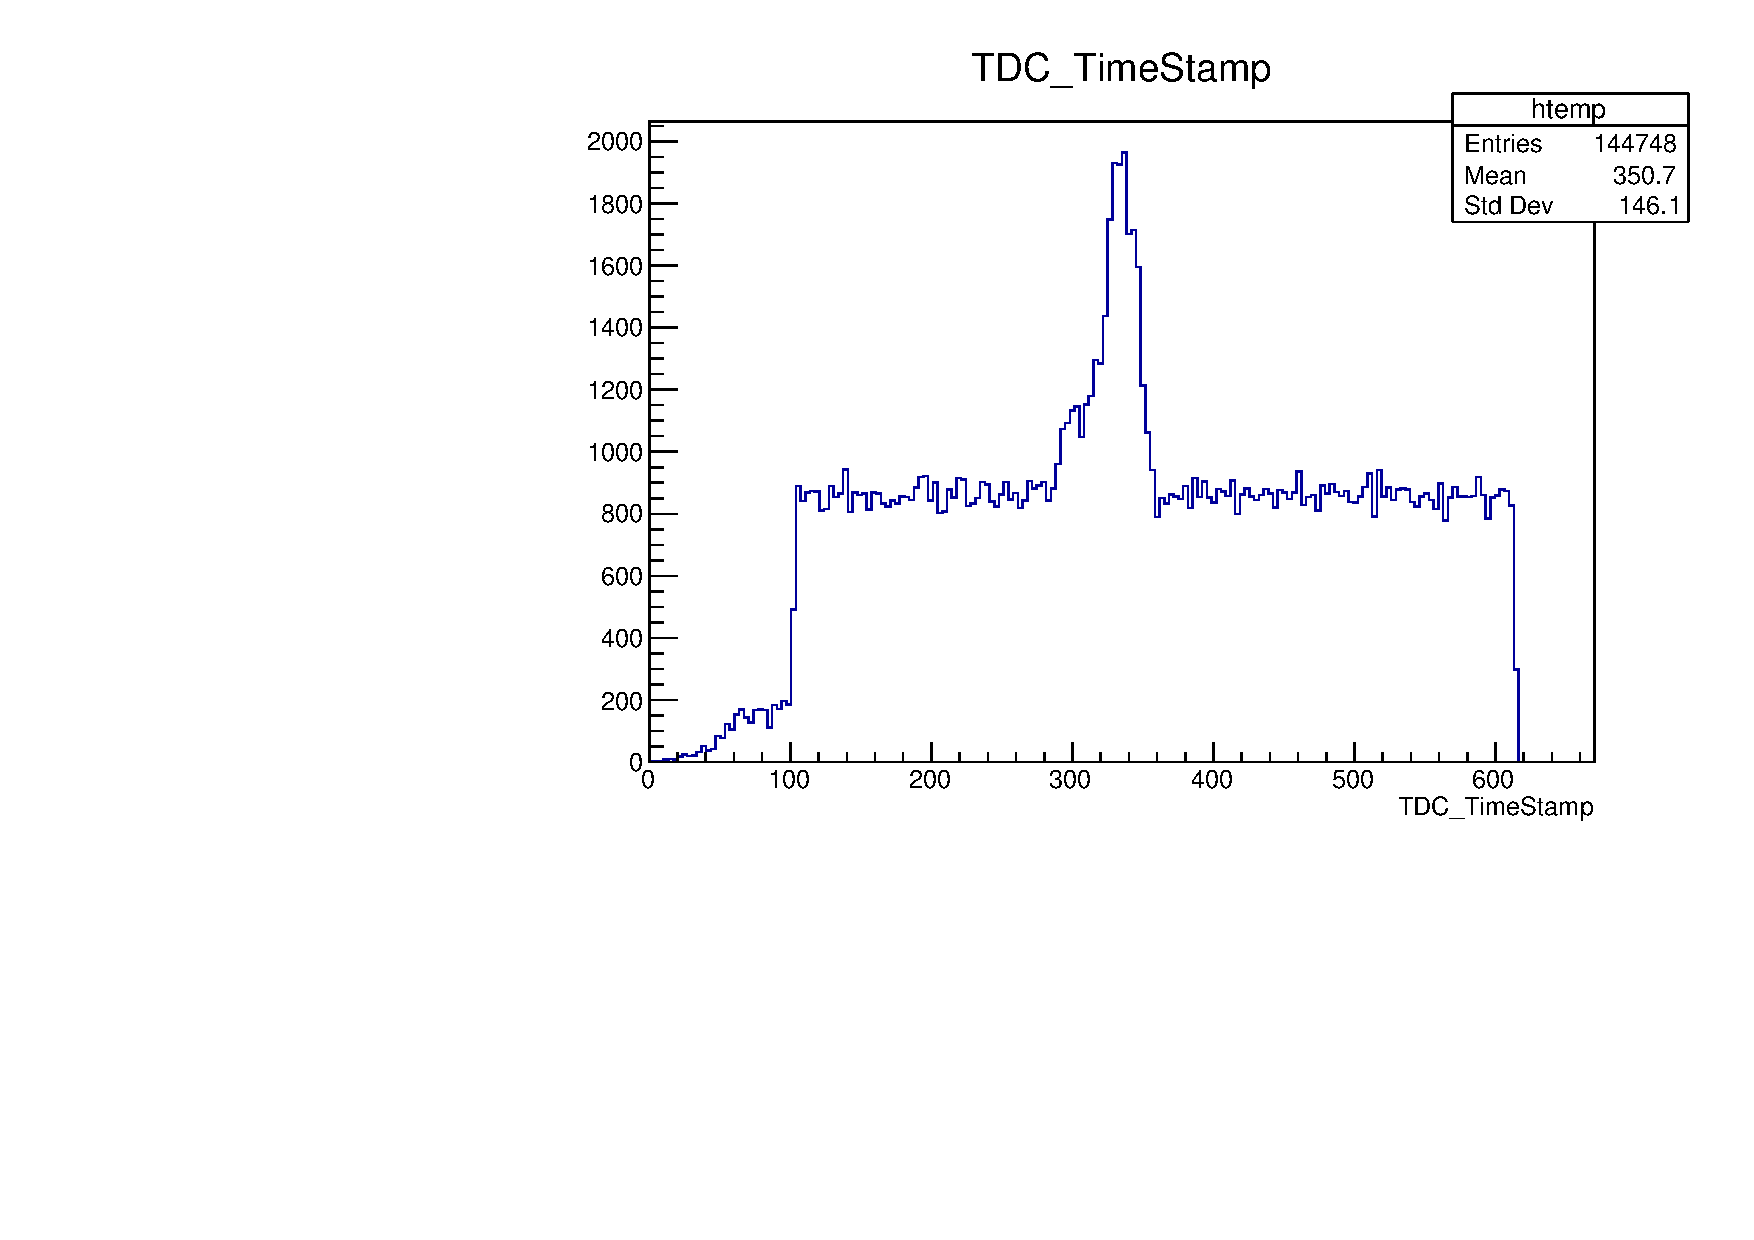
\includegraphics[width = \linewidth]{fig/app2/beam_TS.pdf}
			\caption{\label{fig:TS:A}}
		\end{subfigure}
		\begin{subfigure}{0.5\linewidth}
		    \centering
			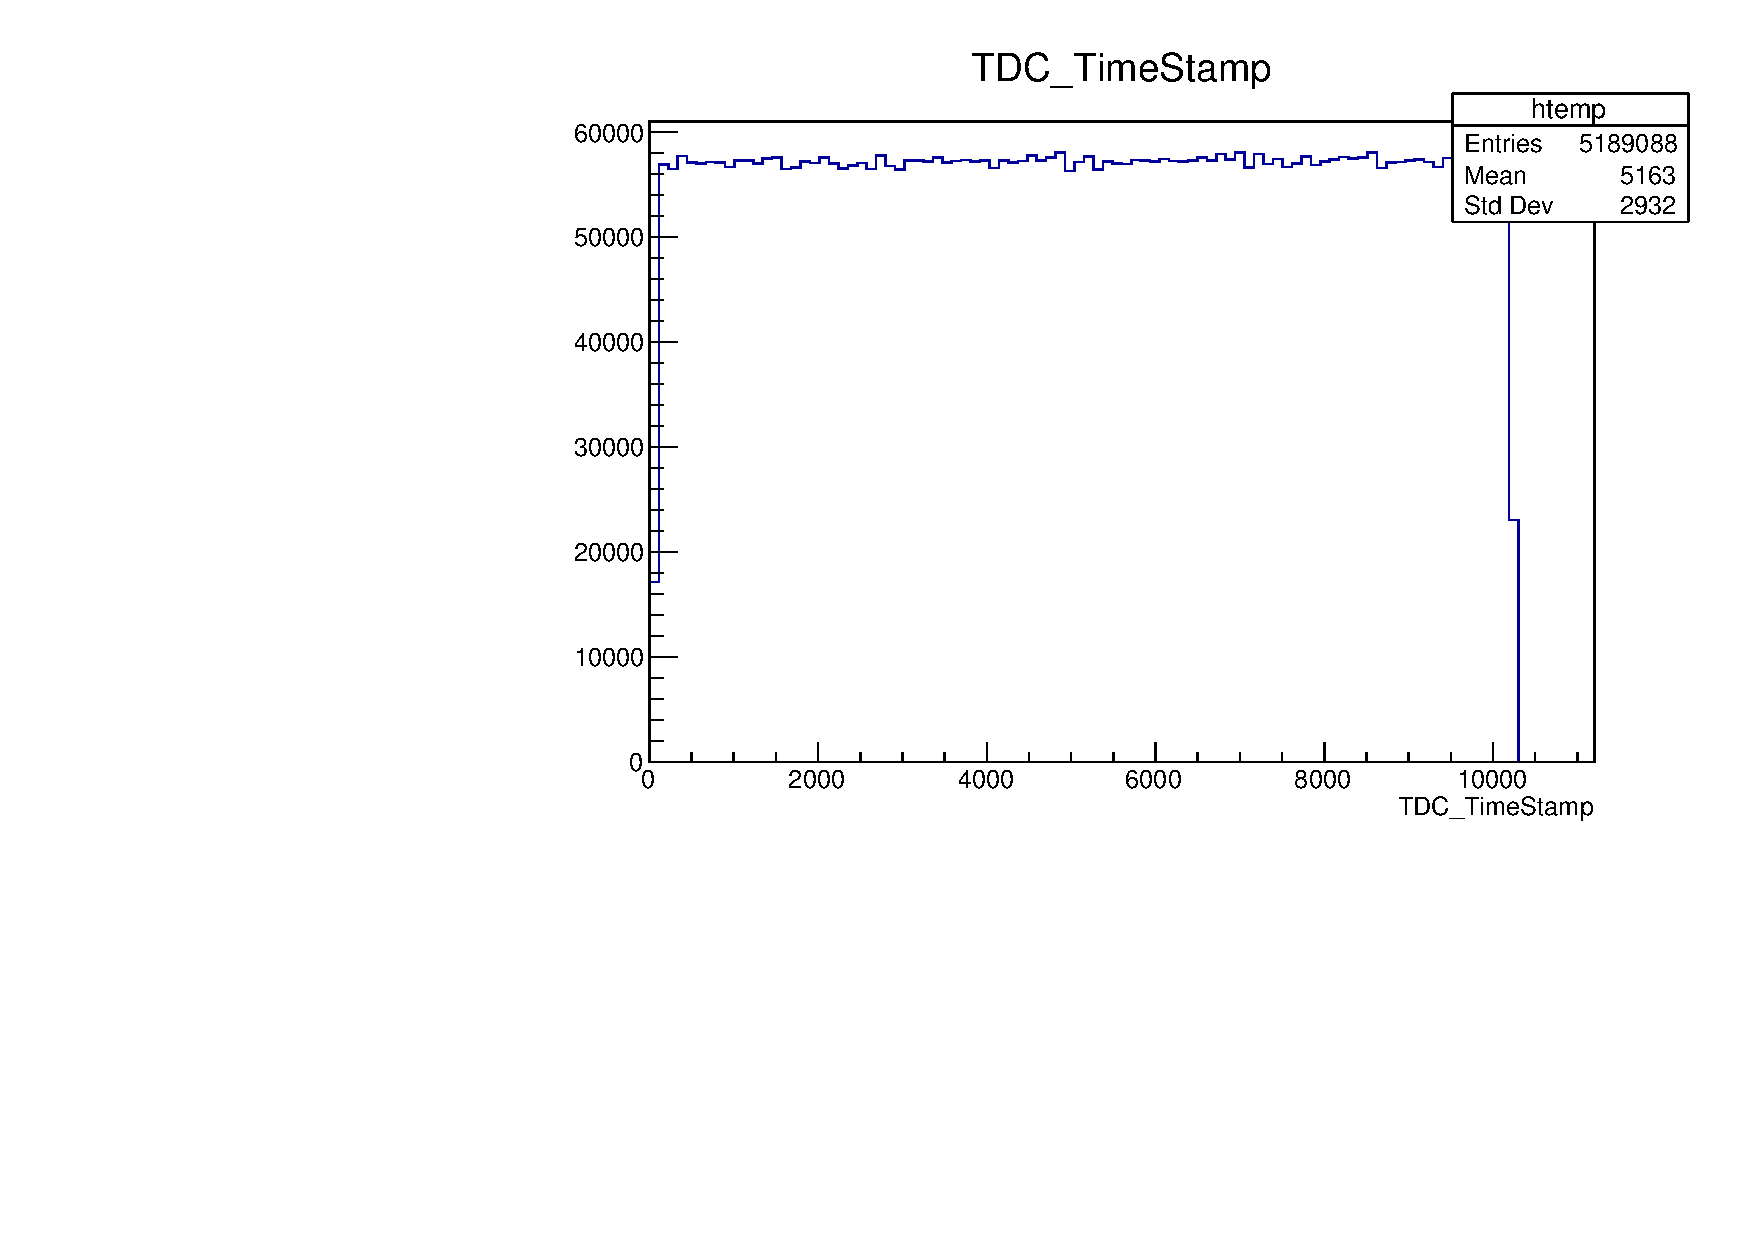
\includegraphics[width = \linewidth]{fig/app2/random_TS.pdf}
			\caption{\label{fig:TS:B}}
		\end{subfigure}
		\caption{\label{fig:TS} Example of expected hit time distributions in the cases of efficiency (Figure~\ref{fig:TS:A}) and noise/gamma rate per unit area (Figure~\ref{fig:TS:B}) measurements as extracted from the raw ROOT files. The unit along the x-axis corresponds to \si{ns}. The fact that "the" muon peak is not well defined in Figure~\ref{fig:TS:A} is due to the contribution of all the RPCs being tested at the same time that don't necessarily have the same signal arrival time. Each individual peak can have an offset with the ones of other detectors. The inconsistancy in the first \SI{100}{ns} of both time distributions is an artefact of the TDCs and are systematically rejected during the analysis.}
	\end{figure}
	
	The ROOT files include a \cppinline{TTree} called \cppinline{RunParameters} containing, among other things, the information related to the type of run. The run type can then be accessed as described by Soucrce Code~\ref{cpp:runtype} and the function \cppinline{IsEfficiencyRun()} is then used to determine if the run file is an efficiency run or, on the contrary, another type of run (noise or gamma measurement).\\
	
	\begin{code}
	\begin{cppcode}
TTree* RunParameters = (TTree*)dataFile.Get("RunParameters");
TString* RunType = new TString();
RunParameters->SetBranchAddress("RunType",&RunType);
RunParameters->GetEntry(0);
	\end{cppcode}
	\captionof{listing}{Access to the run type contained in \cppinline{TTree* RunParameters}.}
	\label{cpp:runtype}
	\vspace{5mm}
	\end{code}
	
	Finally, the data files will have a slightly different content whether it was collected before or after October 2017 and the upgrade of the DAQ software that brought a new information into the ROOT output. This is discussed in Appendix~\ref{app1:ssec:QFlag} and implies that the analysis will differ a little depending on the data format. Indeed, as no information on the data quality is stored, in older data files, the corrections for missing events has to be done at the end of the analysis. The information about the type of data format is stored in the variable \cppinline{bool isNewFormat} by checking the list of branches contained in the data tree via the methods \cppinline{TTree::GetListOfBranches()} and \cppinline{TCollection::Contains()}.
	
	\subsection{Beam time window calculation for efficiency runs}
	\label{app2:ssec:beamwindow}
	
	Knowing the run type is important first of all to know the width of the acquisition window to be used for the rate calculation and finally to be able to seek for muons. Indeed, the peak that appears in the time distribution for each detectors is then fitted to extract the most probable time window in which the tool should look for muon hits. The data outside of this time window in then used to evaluate the noise or gamma background the detector was subbjected to during the data taking. Computing the position of the peak is done calling the function \cppinline{SetBeamWindow()} defined in file \textinline{src/RPCHit.cc} that loops a first time on the data. The data is first sorted in a 3D array of 1D histograms (\cppinline{GIFH1Array}, see \textinline{include/types.h}). Then the location of the highest bin is determined using \cppinline{TH1::GetMaximumBin()} and is used to define a window in which a gaussian fit will be applied to compute the peak width. This window is a \SI{80}{ns} defined by Formula~\ref{eq:fitwindow} around the central bin.
	
	\begin{subequations}
	\label{eq:fitwindow}
	\begin{align}
		t_{center}(ns) & = bin \times width_{bin}(ns)\\
		[t_{low};t_{high}] & = [t_{center} - 40; t_{center} + 40]
	\end{align}
	\end{subequations}
	
	Before the fit is performed, the average number of noise/gamma hits per bin is evaluated using the data outside of the fit window. Excluding the first \SI{100}{ns}, the average number of hits per bin due to the noise or gamma is defined by Formula~\ref{eq:noisehits} after extracting the amount of hits in the time windows $[100;t_{low}]$ and $[t_{high};600]$ thanks to the method \cppinline{TH1::Integral()}. This average number of hits is then subtracted to every bin of the 1D histogram, in order to \textit{clean} it from the noise or gamma contribution as much as possible to improve the fit quality. Bins where $\left\langle n_{hits} \right\rangle$ is greater than the actual bin content are set to 0.
	
	\begin{subequations}
	\label{eq:noisehits}
	\begin{align}
		\Delta t_{noise}(ns) & = 600 \overbrace{- t_{high} + t_{low}}^{-80ns} - 100 = 420ns \\
		\left\langle n_{hits} \right\rangle & = width_{bin}(ns) \times \frac{\sum_{t=100}^{t_{low}}+\sum_{t=t_{high}}^{600}}{\Delta t_{noise}(ns)}
	\end{align}
	\end{subequations}
	
	Finally, the fit parameters are extracted and saved for each detector in 3D arrays of \cppinline{float} (\cppinline{muonPeak}, see \textinline{include/types.h}), a first one for the mean arrival time of the muons, \cppinline{PeakTime}, and a second one for the width of the peak, \cppinline{PeakWidth}. The width is defined as 6$\sigma$ of the gaussian fit. The same settings are applied to every partitions of the same detector. To determine which one of the detector's partitions is directly illuminated by the beam, the peak height of each partition is compared and the highest one is then used to define the peak settings.
	
	\subsection{Data loop and histogram filling}
	\label{app2:ssec:dataloop}
	
	3D arrays of histogram are created to store the data and display it on the DQM of GIF++ webDCS for the use of shifters. These histograms, presented in section~\ref{app2:sssec:ROOT}, are filled while looping on the data. Before starting the analysis loop, it is necessary to control the entry quality for the new file formats featuring \cppinline{QFlag}. If the \cppinline{QFlag} value for this entry shows that 1 TDC or more have a \cppinline{CORRUPTED} flag, then this event is discarded. The loss of statistics is low enough to be neglected. \cppinline{QFlag} is controled using the function \cppinline{IsCorruptedEvent()} defined in \textinline{src/utils.cc}. As explained in Appendix~\ref{app1:ssec:QFlag}, each digit of this integer represent a TDC flag that can be 1 or 2. Each 2 is the sign of a \cppinline{CORRUPTED} state. Then, the data is accessed entry by entry in the ROOT \cppinline{TTree} using \cppinline{RAWData} and each hit in the hit list is assigned to a detector channel and saved in the corresponding histograms. In the first part of the analysis, in which the loop over the ROOT file's content is performed, the different steps are:
	
	\paragraph{1- RPC channel assignment and control:} a check is done on the RPC channel extracted thanks to the mapping via the method \cppinline{Mapping::GetLink()}. If the channel is not initialised and is 0, or if the TDC channel was greater than 5127, the hit is discarded. This means there was a problem in the mapping. Often a mapping problem leads to the crash of the offline tool.
	
	\paragraph{2- Creation of a \cppinline{RPCHit} object:} to easily get the trolley, slot and partition in which the hit has been assigned, this object is particularly helpful.
	
	\paragraph{3- General histograms are filled:} the hit is filled into the time distribution and the general hit distribution histograms, and if the arrival time is within the first \SI{100}{ns}, it is discarded and nothing else happens and the loop proceeds with the next hit in the list.
	
	\paragraph{4- Multiplicity counter:}  the hit multiplicity counter of the corresponding detectors incremented.
	
	\paragraph{5-a- \textit{Effiency runs} - Is the hit within the peak window? :} if the peak is contained in the peak window previously defined in section~\ref{app2:ssec:beamwindow}, the hit is filled into the beam hit profile histogram of the corresponding chamber, added into the list of muon hits and increments the counter of \textit{in time} hits. The term \textit{in time} here refers to the hits that are likely to be muons by arriving in the expected time window. If the hit is outside of the peak window, it is filled into the noise profile histogram of the corresponding detector, added into the list of noise/gamma hits and increments the counter of noise/gamma hits.
	
	\paragraph{5-b- \textit{Noise/gamma rate runs} - Noise histograms are filled:} the hit is filled into the noise profile histogram of the corresponding detector, added into the list of noise/gamma hits and increments the counter of noise/gamma hits.
	
	After the loop on the hit list of the entry is over, the next step is too clusterize the 3D lists filled in the previous steps. A 3D loop is then started over the active trolley, slot and RPC partitions to access these objects. Each \cppinline{NoiseHitList} and \cppinline{MuonHitList}, in case of efficiency run, are clusterized as decribed in section~\ref{app2:ssec:RPCCluster}. There corresponding cluster size and multiplicity histograms are filled at the end of the clustering process. Then, the effiency histogram is filled in case of effieincy run. The selection is simply made by checking whether the RPC detected signals in the peak window during this event. Nevertheless, it is useful to highlight that at this level, it is not possible yet to discriminate in between a muon hit and noise or gamma hit. Thus, \cppinline{MuonCSize_H}, \cppinline{MuonCMult_H} and \cppinline{Efficiency0_H} are subjected to noise and gamma contamination. This contamination will be estimated and corrected at the moment the results will be written into output CSV files. Finally, the loop ends on the filling of the general hit multiplicity histogram.
	
	\subsection{Computation of the final results}
	\label{app2:ssec:results}
	
	As mentioned in section~\ref{app2:ssec:output}, the analysis of DAQ data provides the user with 3 CSV files and a ROOT file associated to each and every ROOT data file. The fourth CSV file is provided by the extraction of the CEAN main frame data monitored during data tacking and will be discussed later. After looping on the data in the previous part of the analysis macro, the output files are created and a 3D loop on each RPC readout partitions is started to extract the histograms parameters and compute the final results.\\
	
	\begin{figure}[H]
        \centering
		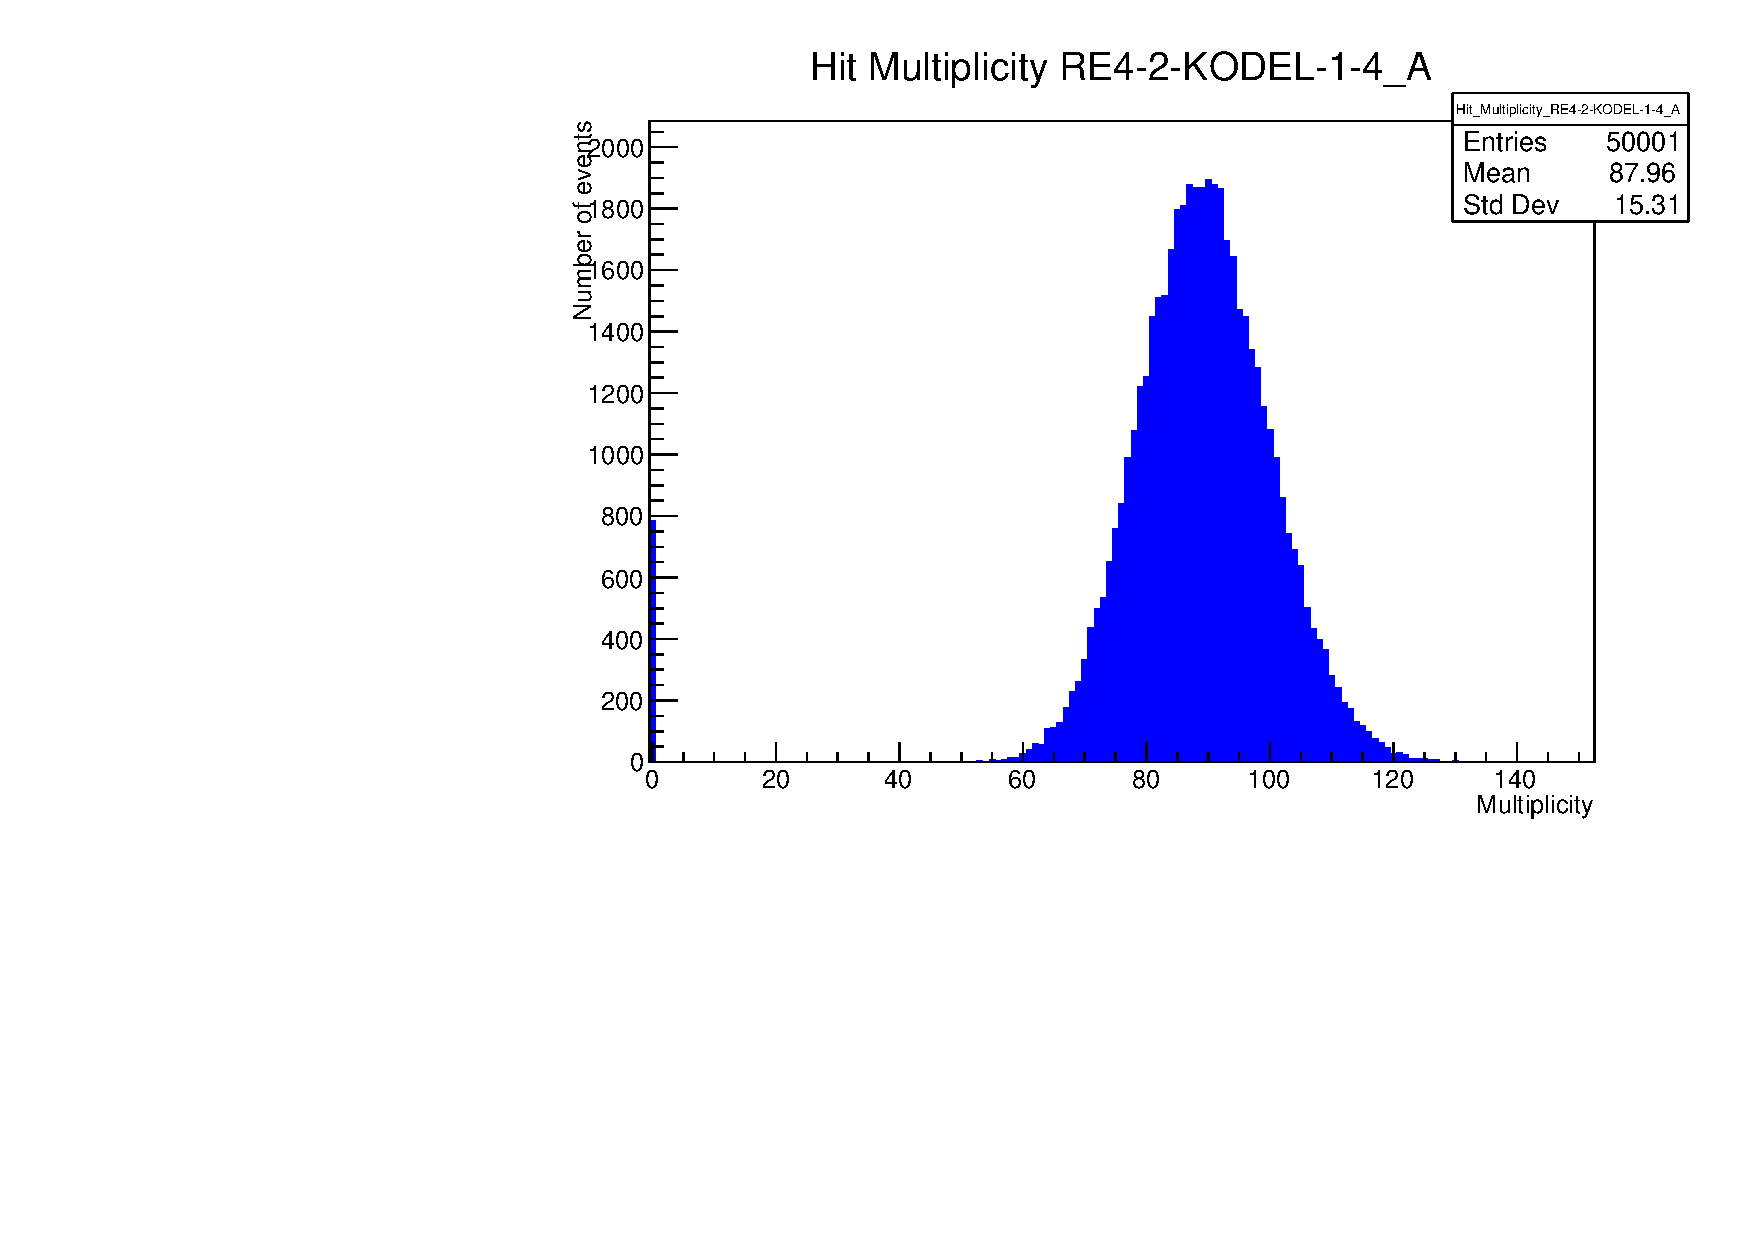
\includegraphics[width = 0.7\linewidth]{fig/app1/No_Qflag_nhits_KODEL.pdf}
		\caption{\label{fig:corrupted} The effect of the quality flag is explained by presenting the reconstructed hit multiplicity of a data file without \cppinline{Quality_flag}. The artificial high content of bin 0 is the effect of corrupted data.}
	\end{figure}
	
	\paragraph{Corrupted data estimation :} In case of old data format files, not containing any quality flag, it is need to estimate the amount of corrupted data via a fit as the corrupted data will always fill events with a fake "0 multiplicity". Indeed, as no hits were stored in the DAQ ROOT files, these events artificially contribute to fill the bin corresponding to a null multiplicity, as shown in Figure~\ref{fig:corrupted}.
	
\clearpage{\pagestyle{empty}\cleardoublepage}